%! TEX program = xelatex
\documentclass[tikz, class=report]{standalone}
\usepackage[lining]{ebgaramond}%[StylisticSet={7,9}]
\usepackage[math-style=ISO, bold-style=ISO]{unicode-math}
\setmathfont{Garamond-Math.otf}
\usepackage{pgfplots}
\usepackage{import}
\makeatletter
  \def\input@path{%
    {../tex/}
    {../../tex/}
    {../../../tex/}
    {../../../../tex/}
  }
\makeatother


\def\dist{3}
\def\hoff{-1.7}

\begin{document}
  \begin{tikzpicture}

    \node[rotate=90] at (0,1.8) {
\includegraphics[height=15cm, trim=5 0 0 0, clip]{data/map-dist/probability-scale.pdf}};
    \node at (-5.7,2.2) {\small $10^{-1}$};
    \node at (-2.4,2.2) {\small $10^{-2}$};
    \node at ( 1.0,2.2) {\small $10^{-3}$};
    \node at (+4.3,2.2) {\small $10^{-4}$};
    \node at (+7.6,2.2) {\small $10^{-5}$};

    \node at (-2*\dist,0) {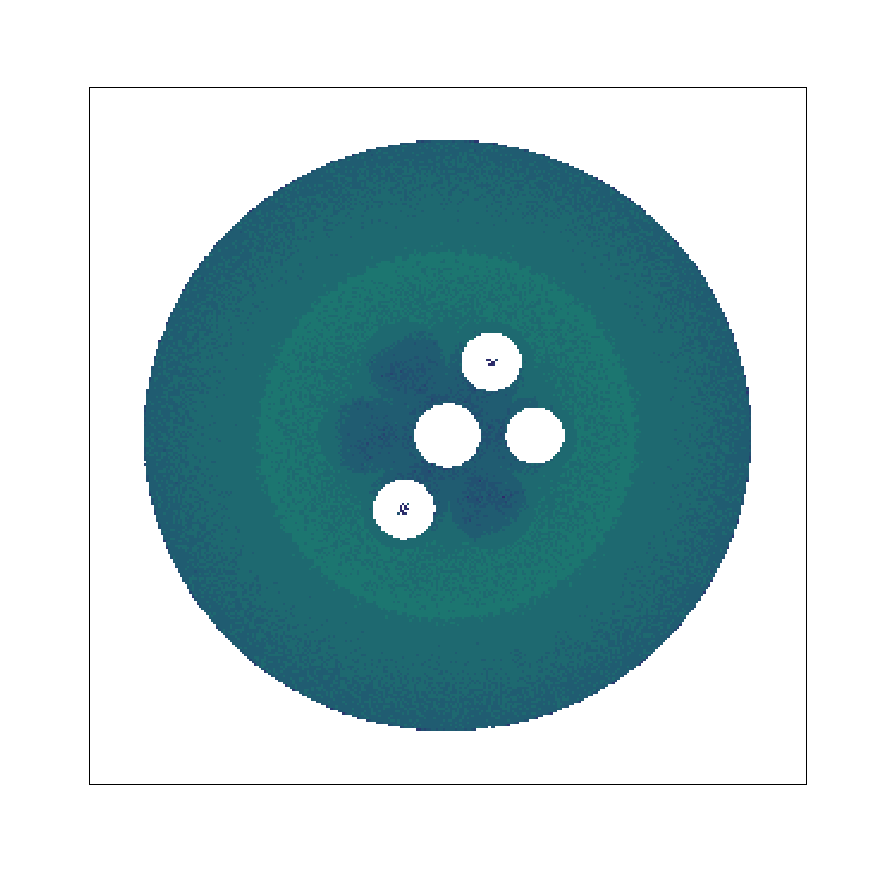
\includegraphics[width=3cm, trim=140 140 140 140, clip]{data/map-dist/gerda-larmap-2nufit-20200803-d0p50-pcanorm.png}};
    \node at (-1*\dist,0) {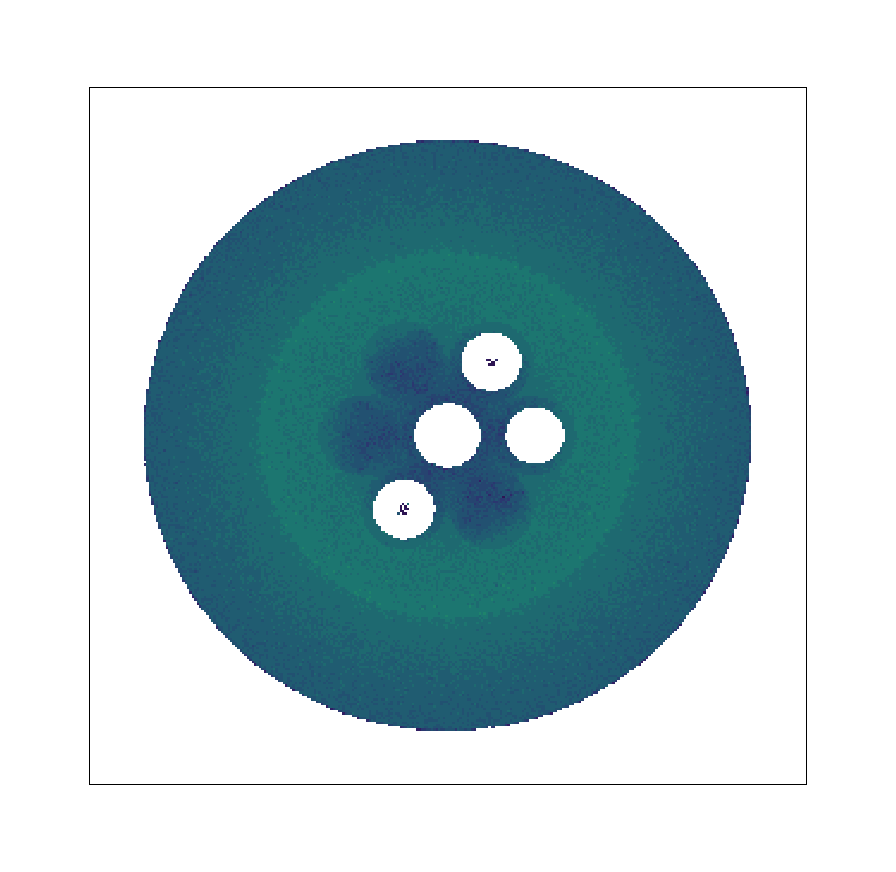
\includegraphics[width=3cm, trim=140 140 140 140, clip]{data/map-dist/gerda-larmap-2nufit-20200803-d0p80-pcanorm.png}};
    \node at ( 0*\dist,0) {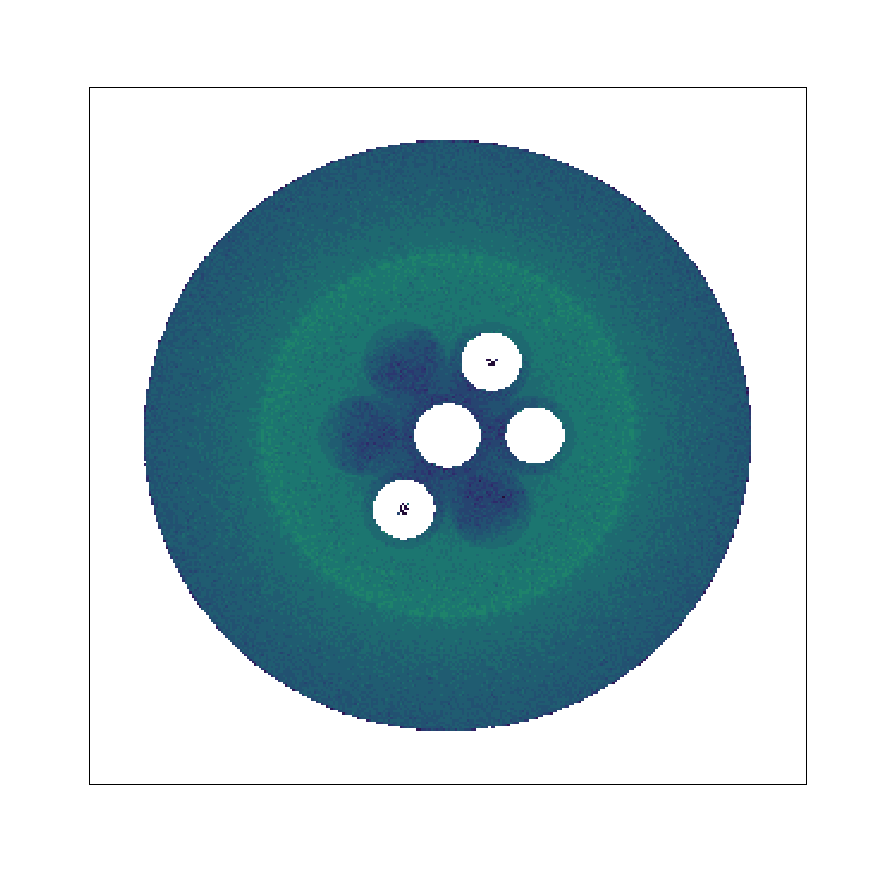
\includegraphics[width=3cm, trim=140 140 140 140, clip]{data/map-dist/gerda-larmap-2nufit-20200803-pcanorm.png}};
    \node at (+1*\dist,0) {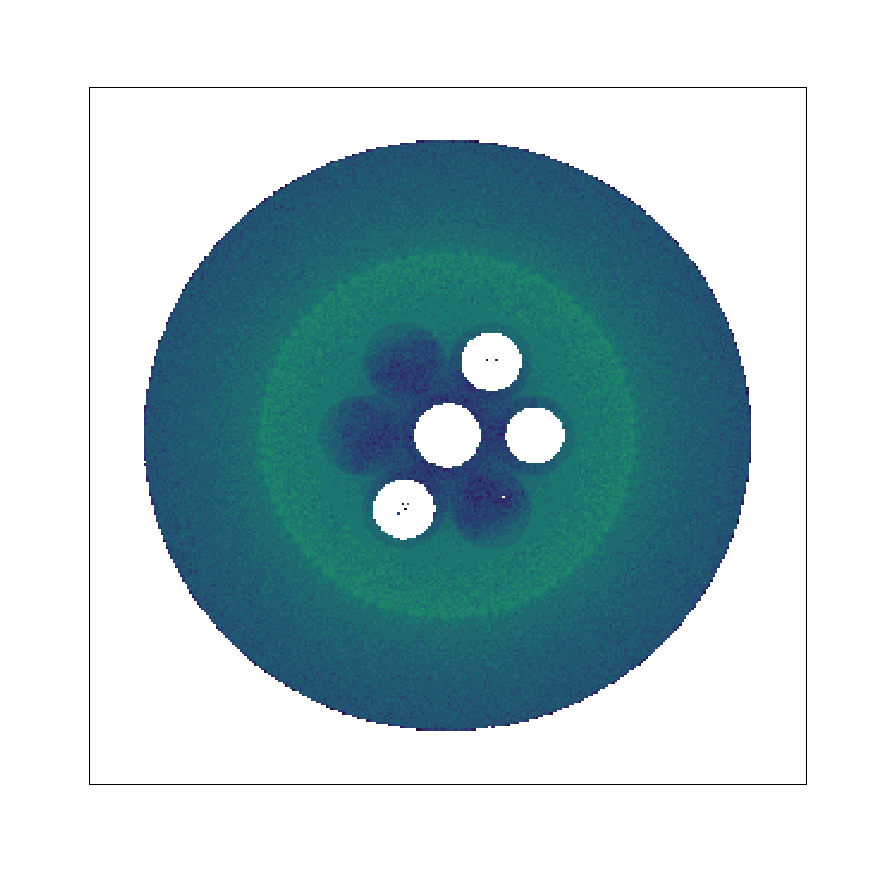
\includegraphics[width=3cm, trim=140 140 140 140, clip]{data/map-dist/gerda-larmap-2nufit-20200803-d1p20-pcanorm.png}};
    \node at (+2*\dist,0) {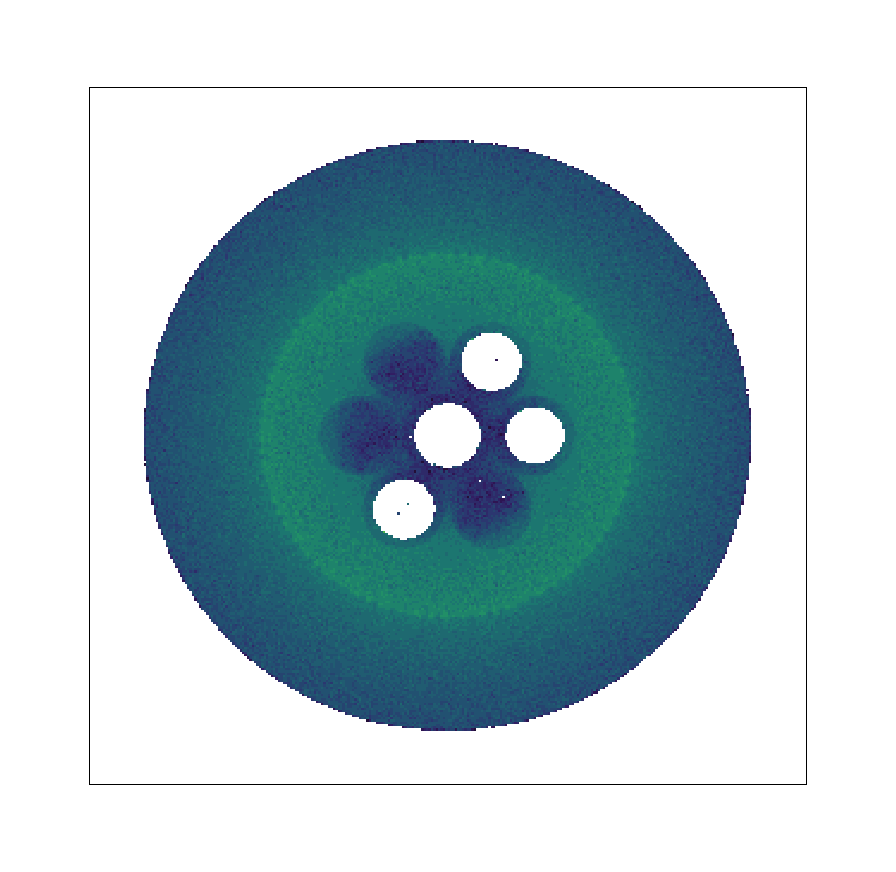
\includegraphics[width=3cm, trim=140 140 140 140, clip]{data/map-dist/gerda-larmap-2nufit-20200803-d1p50-pcanorm.png}};

    \node at (-2*\dist,\hoff) {$a=0.5$};
    \node at (-1*\dist,\hoff) {$a=0.8$};
    \node at ( 0*\dist,\hoff) {$a=1.0$};
    \node at (+1*\dist,\hoff) {$a=1.2$};
    \node at (+2*\dist,\hoff) {$a=1.5$};

  \end{tikzpicture}
\end{document}
